\documentclass[12pt,a4paper]{article}

\usepackage[utf8]{inputenc}
\usepackage[T1]{fontenc}
\usepackage[brazil]{babel}
\usepackage{mathptmx}
\usepackage[a4paper,left=2.5cm,right=2.5cm,top=2.5cm,bottom=2.5cm]{geometry}
\usepackage{graphicx}
\usepackage{booktabs}
\usepackage{array}
\usepackage{amsmath}
\usepackage{microtype}
\usepackage{caption}
\usepackage{float}
\usepackage{fancyhdr}
\usepackage{titlesec}
\usepackage[round,authoryear]{natbib}
\usepackage[hidelinks]{hyperref}

\graphicspath{{figuras/}}
\emergencystretch=2em
\setlength{\parindent}{0.75cm}
\setlength{\parskip}{0pt}
\linespread{1.0}
\setlength{\headheight}{25pt}
\setlength{\headsep}{12pt}
\setlength{\footskip}{25pt}

\pagestyle{fancy}
\fancyhf{}
\fancyhead[L]{\fontsize{8.5}{9.5}\selectfont\itshape III MCSM\\13--15 de agosto de 2026}
\fancyfoot[C]{\fontsize{8}{9}\selectfont\itshape Anais do III MCSM -- Modelagem Computacional do Sertão Mineiro - 2026}
\renewcommand{\headrulewidth}{0pt}
\renewcommand{\footrulewidth}{0pt}

\titleformat{\section}
  {\normalfont\bfseries}
  {\thesection.}{0.75cm}{\MakeUppercase}
\titlespacing*{\section}{0pt}{12pt}{12pt}
\titleformat{\subsection}
  {\normalfont\bfseries}
  {\thesubsection}{0.75cm}{}
\titlespacing*{\subsection}{0pt}{12pt}{12pt}

\captionsetup{
  font=normalfont,
  labelfont=normalfont,
  labelsep=colon,
  justification=centering,
  singlelinecheck=true,
  skip=8pt
}
\renewcommand{\refname}{REFERÊNCIAS}
\setlength{\bibsep}{3pt}
\bibpunct{(}{)}{;}{a}{,}{,}

\newcommand{\autor}[2]{\noindent\textbf{#1}$^{1}$ - #2\par}

\begin{document}

\begin{center}
  
\includegraphics[width=0.88\textwidth]{cabecalho_iii_mcsm.png}
\end{center}

\vspace{8pt}

\begin{center}
\begin{minipage}{0.96\textwidth}
\centering\bfseries
PREVISÃO MENSAL DE IRRADIÂNCIA GLOBAL HORIZONTAL EM\\
LOCALIDADES DE FÁBRICAS DE VEÍCULOS ELÉTRICOS COM UMA\\
APROXIMAÇÃO DO DEEPNPTS
\end{minipage}
\end{center}

\vspace{12pt}

\autor{Gustavo de Melo Nascimento}{g239679@dac.unicamp.br}
\autor{Thales Wulfert Cabral}{t264377@dac.unicamp.br}
\autor{Gustavo Fraidenraich}{gfraiden@unicamp.br}
\noindent$^{1}$Faculdade de Engenharia Elétrica e de Computação, Universidade Estadual de Campinas -- Campinas, SP, Brasil

\vspace{24pt}

\noindent\textbf{\textit{Abstract.}} \textit{Este artigo apresenta um sistema para previsão mensal da Irradiância Global Horizontal (GHI) em dez localidades associadas a fábricas de veículos elétricos. Foram utilizados dados da National Solar Radiation Database, produto GOES Aggregated PSM v4, entre 2019 e 2024. As observações, coletadas em intervalos de 60 minutos e processadas como médias diárias, foram agregadas por mês civil, quantizadas em 128 níveis, normalizadas e organizadas em atributos temporais para prever o mês seguinte. O método proposto é uma aproximação experimental inspirada no DeepNPTS, que combina similaridade entre padrões históricos e ponderação por recência. A avaliação adotou divisão cronológica de 80\% para treinamento e 20\% para teste. Entre sete modelos, a aproximação obteve o menor erro médio: MAE de 12,96 W/m$^2$, RMSE de 16,39 W/m$^2$, $R^2$ de 0,916 e nRMSE de 8,10\%. Em relação à RNN, melhor referência média, houve redução de 12,50\% no MAE e 10,07\% no RMSE.}

\vspace{12pt}

\noindent\textbf{\textit{Keywords:}} \textit{Irradiância solar, GHI, Previsão mensal, Séries temporais, DeepNPTS}

\section{Introdução}

A expansão da geração fotovoltaica aumenta a necessidade de estimar antecipadamente a disponibilidade do recurso solar. Como a potência produzida depende da irradiância incidente, erros de previsão afetam o planejamento operacional, o dimensionamento de instalações e a integração da geração à rede \citep{antonanzas2016,voyant2017,yang2018}. Este trabalho considera a Irradiância Global Horizontal (GHI), definida por

\begin{equation}
  \mathrm{GHI}=\mathrm{DHI}+\mathrm{DNI}\cos(\theta_z),
  \label{eq:ghi}
\end{equation}

\noindent em que DHI é a irradiância difusa horizontal, DNI é a irradiância direta normal e $\theta_z$ é o ângulo zenital solar \citep{duffie2013}. A GHI reúne as componentes direta e difusa e permite comparar localidades sob a mesma referência física, em W/m$^2$ \citep{sengupta2018}.

Em escala mensal, a agregação reduz oscilações meteorológicas de curta duração e evidencia sazonalidade e tendências do recurso solar. Entretanto, cada ano acrescenta somente doze observações, tornando a tarefa um problema de séries temporais curtas. Métodos tabulares e redes neurais são amplamente empregados na previsão solar \citep{sobri2018}. Entre eles, o XGBoost representa relações não lineares por árvores impulsionadas \citep{chen2016}, enquanto RNNs e LSTMs tratam dependências sequenciais \citep{hochreiter1997}.

O Deep Non-Parametric Time Series Forecaster (DeepNPTS) aprende probabilidades de amostragem sobre observações históricas sem impor uma família paramétrica fixa à distribuição preditiva \citep{rangapuram2023}. Essa reutilização de padrões observados é atraente quando há poucas amostras mensais. Assim, o objetivo deste estudo é avaliar um sistema inspirado nesse princípio para prever a GHI média do mês seguinte em dez localidades associadas a fábricas de veículos elétricos. A contribuição é uma comparação homogênea entre sete modelos, com o mesmo processamento, corte temporal e conjunto de métricas. O rótulo ``DeepNPTS'' empregado adiante identifica a aproximação experimental descrita na Seção~\ref{sec:metodo}, e não uma reprodução integral da arquitetura original.

\section{Metodologia}
\label{sec:metodo}

\subsection{Dados e protocolo experimental}

Foram utilizados dados da National Solar Radiation Database (NSRDB), atualmente mantida pelo National Laboratory of the Rockies (NLR, anteriormente NREL), no produto GOES Aggregated PSM v4 \citep{nlr2026}. A consulta abrangeu 1 de janeiro de 2019 a 31 de dezembro de 2024, com intervalo de 60 minutos. O fluxo armazenou médias diárias e, posteriormente, calculou a média de cada mês civil.

As dez localidades são: BYD Camaçari, BMW San Luis Potosí, Ford Rouge, GM Factory Zero, Hyundai Metaplant Georgia, Lucid AMP 1 Casa Grande, Rivian Normal e as unidades Tesla de Fremont, Nevada e Texas. Cada série foi ordenada e verificada quanto a cobertura temporal, duplicidades, ausências, valores negativos e consistência geográfica. A GHI foi mantida em W/m$^2$.

Após a criação dos atributos, cada localidade forneceu 60 exemplos supervisionados, com alvos entre janeiro de 2020 e dezembro de 2024. A divisão cronológica destinou 48 exemplos ao treinamento e 12 ao teste, correspondentes aos meses de 2024, sem embaralhamento. Cada entrada de teste utilizou apenas o histórico disponível até o instante da previsão, e os modelos permaneceram fixos durante o teste. A Tabela~\ref{tab:config} resume as condições principais.

\begin{table}[htbp]
\centering
\caption{Configuração do experimento mensal.}
\label{tab:config}
\renewcommand{\arraystretch}{1.05}
\begin{tabular}{>{\raggedright\arraybackslash}p{4.0cm}>{\raggedright\arraybackslash}p{10.3cm}}
\toprule
\textbf{Item} & \textbf{Configuração} \\
\midrule
Dados & NSRDB/NLR, GOES Aggregated PSM v4, GHI em W/m$^2$, 2019--2024. \\
Previsão & Um mês à frente; 48 exemplos de treino e 12 de teste por localidade. \\
Pré-processamento & Quantização em 128 níveis e normalização min--max ajustadas somente no treino. \\
Atributos & Defasagens de 1, 2, 3 e 6 meses; médias móveis de 3, 6 e 12 meses. \\
Modelos & XGBoost, MLP, RNN, LSTM, DilatedRNN exp., DeepAR exp. e DeepNPTS aprox. \\
Reprodutibilidade & Semente 42; uma execução por modelo e localidade. \\
\bottomrule
\end{tabular}
\end{table}

\subsection{Pré-processamento e modelos}

Os limites da quantização e da transformação min--max foram estimados somente com o conjunto de treinamento e reutilizados no teste. As defasagens e médias móveis formaram os pares $(X_{\ell,t},y_{\ell,t+1})$, em que $\ell$ identifica a localidade. Os concorrentes foram configurados conforme os registros experimentais: XGBoost com 300 estimadores, profundidade 3 e taxa 0,05; MLP com camadas ocultas de 64 e 32 neurônios; e RNN/LSTM com 32 unidades recorrentes, camada densa de 16 neurônios e saída sigmoidal. As redes utilizaram Adam, taxa 0,001, MSE, 80 épocas e lote 32. A DilatedRNN experimental combinou ramos com dilatações 1, 2 e 4, e o DeepAR experimental empregou LSTM com saída gaussiana \citep{chang2017,salinas2020}.

Na aproximação do DeepNPTS, o vetor corrente é comparado aos históricos candidatos. Similaridade e recência definem os pesos usados na previsão pontual:

\begin{equation}
\begin{aligned}
  \widehat{y}_{\ell,t+1}
  &=\frac{\sum_{j\in\mathcal H_{\ell,t}}w_{t,j}y_{\ell,j+1}}
  {\sum_{j\in\mathcal H_{\ell,t}}w_{t,j}},\\
  w_{t,j}&=\exp\!\left[-d(X_{\ell,t},X_{\ell,j})/\tau\right]\gamma^{t-j},
\end{aligned}
\label{eq:deepnpts}
\end{equation}

\noindent em que $\mathcal H_{\ell,t}$ reúne os históricos, $d(\cdot)$ é a distância euclidiana, $\tau=0{,}08$ controla a concentração e $\gamma=0{,}995$ pondera a recência. Foram considerados até $k=80$ vizinhos, limitados aos 48 exemplos de treino. Ao contrário do DeepNPTS canônico, essa implementação não treina uma rede global nem otimiza um escore probabilístico: os pesos da Equação~\ref{eq:deepnpts} são calculados diretamente em cada série.

\subsection{Métricas e seleção}

Sejam $y_i$ a GHI real, $\widehat y_i$ a previsão, $\bar y$ a média observada e $n$ o número de meses de teste. Foram calculados MAE, MSE, RMSE, $R^2$ e nRMSE. Para concisão, as métricas centrais são

\begin{equation}
\begin{aligned}
 \mathrm{MAE}&=\frac{1}{n}\sum_{i=1}^{n}|y_i-\widehat y_i|,\\
 \mathrm{RMSE}&=\sqrt{\frac{1}{n}\sum_{i=1}^{n}(y_i-\widehat y_i)^2},\\
 \mathrm{nRMSE}(\%)&=100\,\mathrm{RMSE}/\bar y.
\end{aligned}
\label{eq:metricas}
\end{equation}

O MAE em W/m$^2$ definiu o vencedor por ser diretamente interpretável e menos sensível a erros extremos do que o RMSE \citep{hyndman2006}. Para cada modelo $m$, calculou-se $\overline{\mathrm{MAE}}_m$ entre as dez localidades; selecionou-se $m^*=\arg\min_m\overline{\mathrm{MAE}}_m$.

\section{Resultados e discussão}
\label{sec:resultados}

A Tabela~\ref{tab:metricas} apresenta as médias das métricas nas dez localidades, ordenadas pelo MAE. A aproximação do DeepNPTS obteve o menor MAE (12,96 W/m$^2$), o menor RMSE (16,39 W/m$^2$), o maior $R^2$ (0,916) e o menor nRMSE (8,10\%). Portanto, a seleção pelo MAE não contradiz os demais indicadores.

\begin{table}[htbp]
\centering
\caption{Métricas médias mensais dos modelos avaliados.}
\label{tab:metricas}
\renewcommand{\arraystretch}{1.04}
\setlength{\tabcolsep}{6pt}
\begin{tabular}{lrrrrr}
\toprule
\textbf{Modelo} & \textbf{MAE} & \textbf{MSE} & \textbf{RMSE} & \textbf{$R^2$} & \textbf{nRMSE} \\
 & \textbf{W/m$^2$} & \textbf{W$^2$/m$^4$} & \textbf{W/m$^2$} & & \textbf{\%} \\
\midrule
DeepNPTS aprox. & 12,96 & 281,29 & 16,39 & 0,916 & 8,10 \\
RNN & 14,81 & 363,32 & 18,23 & 0,878 & 8,97 \\
XGBoost & 15,23 & 415,07 & 19,41 & 0,875 & 9,70 \\
DilatedRNN exp. & 15,25 & 380,90 & 18,73 & 0,878 & 9,29 \\
MLP & 16,13 & 412,61 & 19,70 & 0,861 & 9,58 \\
LSTM & 20,60 & 659,72 & 24,69 & 0,785 & 11,99 \\
DeepAR exp. & 61,02 & 5038,27 & 68,57 & 0,010 & 34,21 \\
\bottomrule
\end{tabular}
\end{table}

Em relação à RNN, melhor referência média, a aproximação reduziu o MAE em 12,50\% e o RMSE em 10,07\%. A diferença para o DeepAR experimental foi mais ampla: redução de 78,76\% no MAE. Esse resultado sugere que a configuração probabilística adotada não se ajustou às séries mensais com apenas 48 exemplos de treinamento. A Figura~\ref{fig:mae_medio} evidencia tanto a vantagem do método proposto quanto a distância do DeepAR em relação ao grupo principal.

\begin{figure}[htbp]
\centering
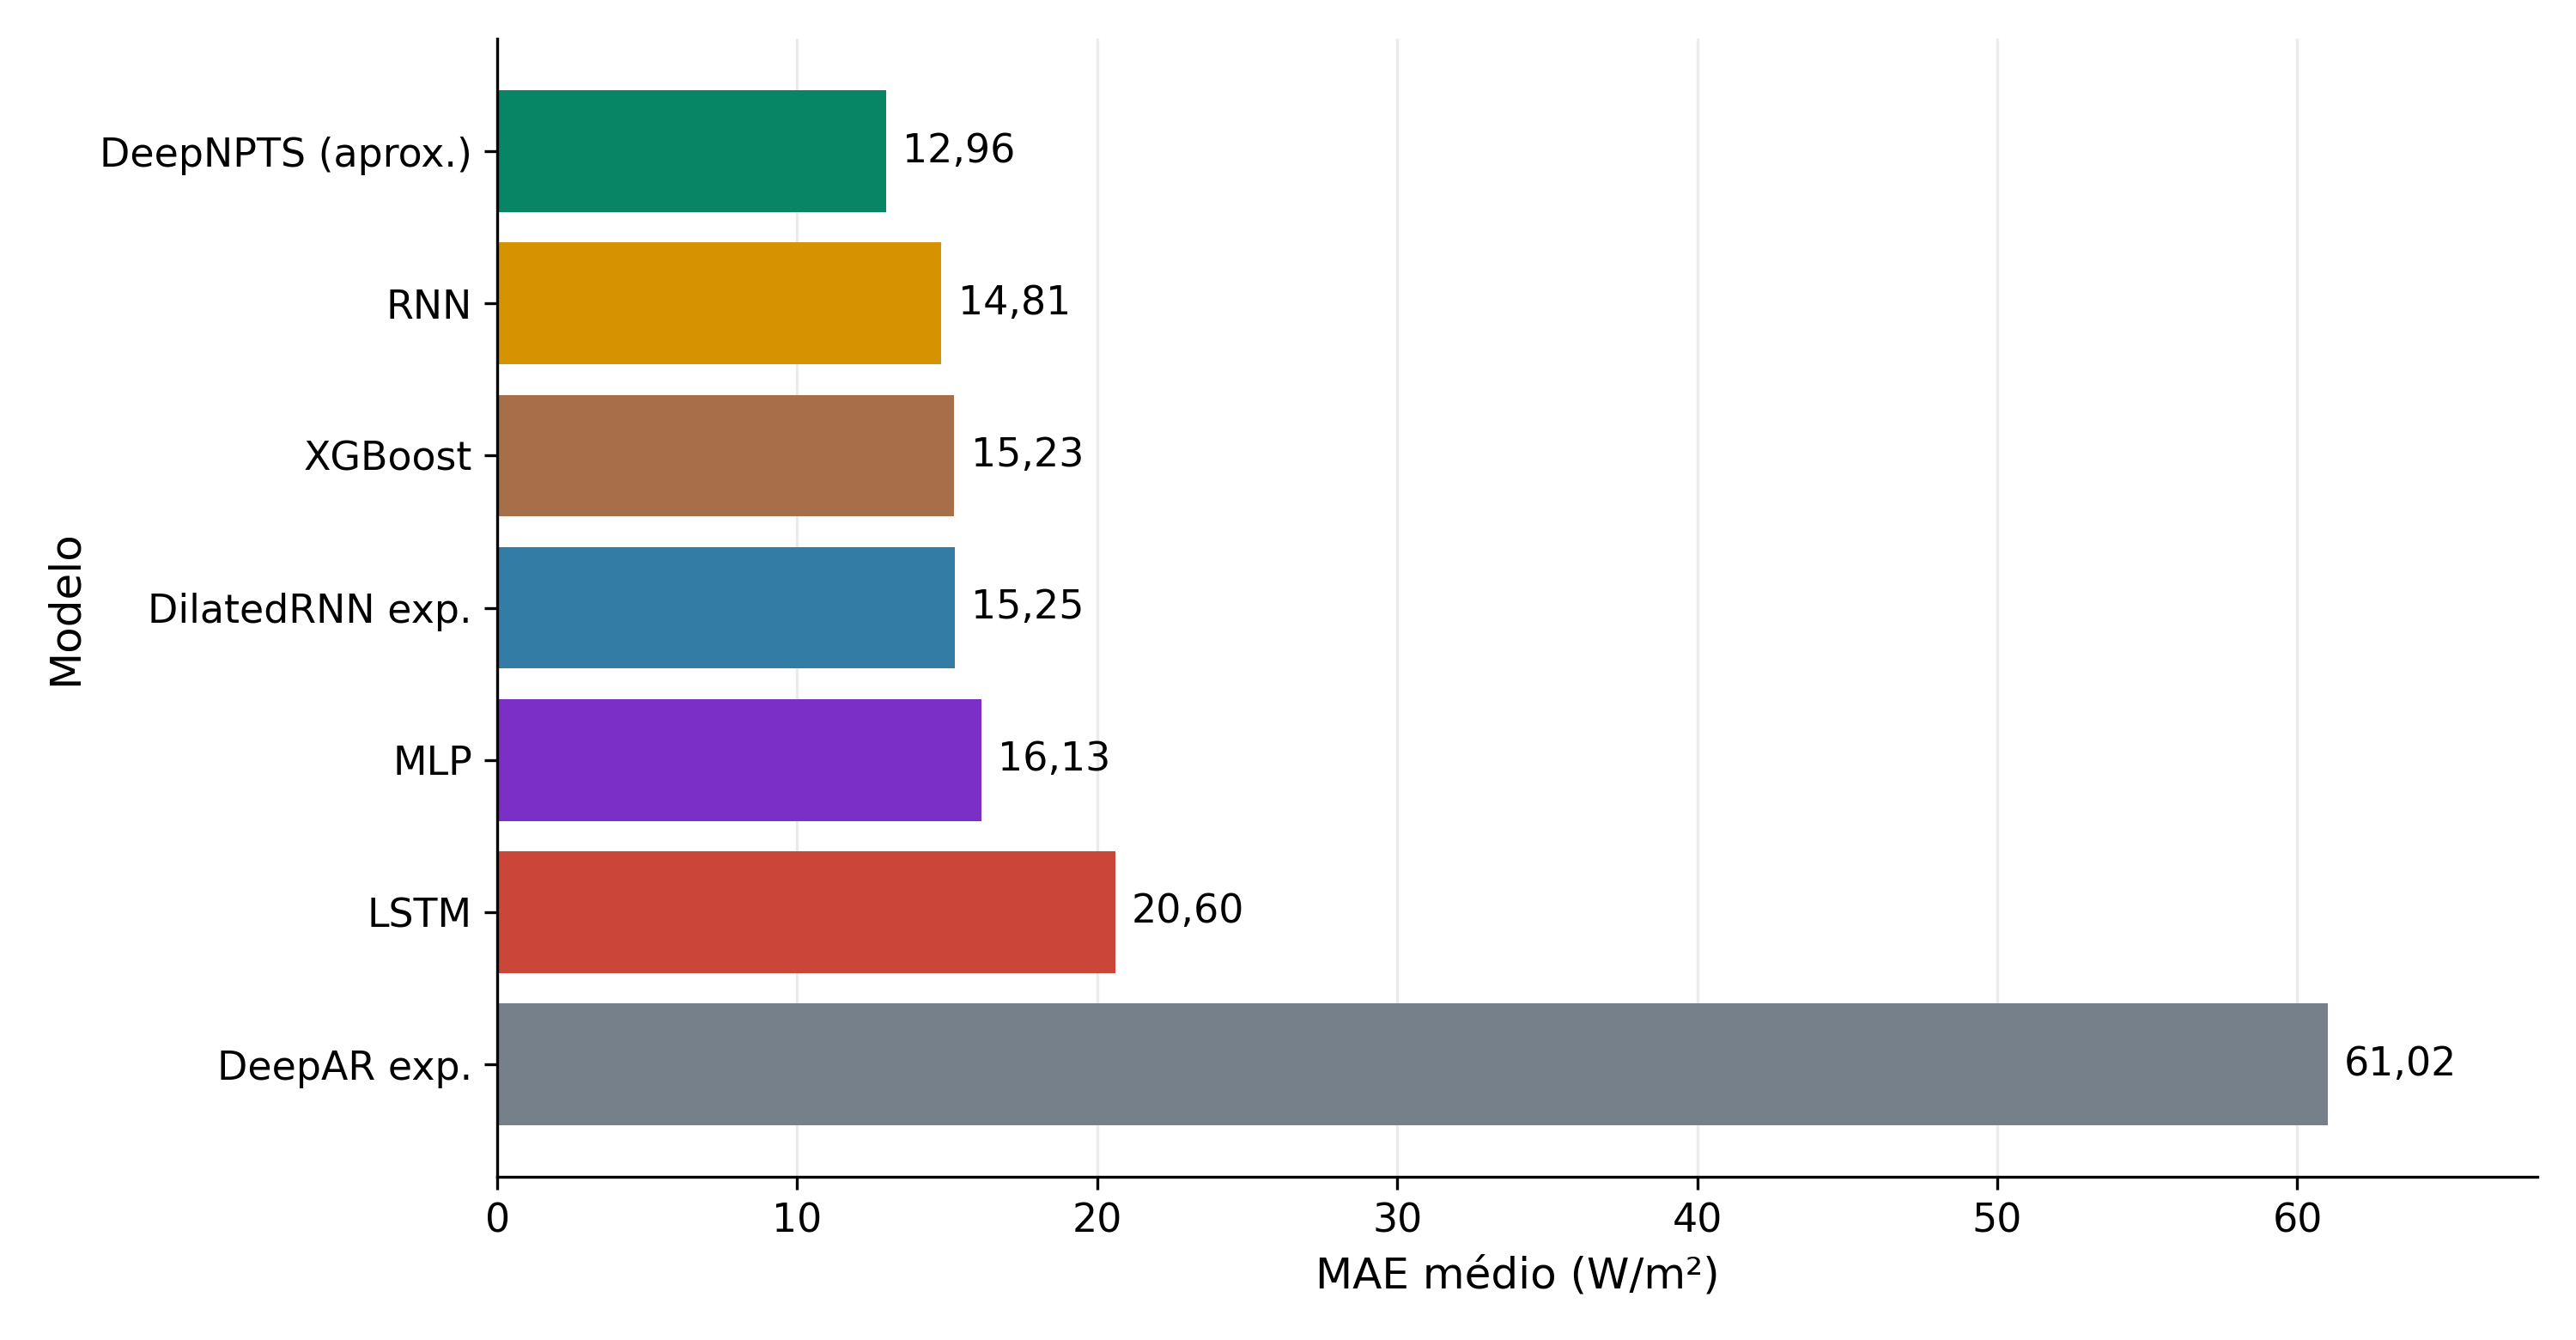
\includegraphics[width=0.84\textwidth]{mae_medio_modelos.png}
\caption{MAE médio dos modelos nas dez localidades; valores menores indicam melhor desempenho.}
\label{fig:mae_medio}
\end{figure}

A análise individual mostra que a aproximação venceu em cinco localidades: BMW San Luis Potosí, BYD Camaçari, Hyundai Metaplant Georgia, Rivian Normal e Tesla Texas. A RNN venceu em Ford Rouge, GM Factory Zero e Tesla Fremont; o XGBoost, em Lucid Casa Grande; e a DilatedRNN experimental, em Tesla Nevada. O melhor MAE do método proposto ocorreu na Tesla Texas (9,50 W/m$^2$), e o pior, na BMW San Luis Potosí (18,65 W/m$^2$).

Na Tesla Texas, a redução frente à MLP, melhor concorrente local, foi de 37,23\%. Em contraste, o XGBoost obteve 5,61 W/m$^2$ na Lucid Casa Grande, contra 10,40 W/m$^2$ da aproximação. A Figura~\ref{fig:mae_localidades} confirma que o método é robusto em média, mas não domina todas as condições regionais.

\newpage
Na série de Camaçari, ambos os métodos acompanharam a redução de GHI no meio do ano e a recuperação no último trimestre. A aproximação apresentou MAE de 13,85 W/m$^2$, ante 16,74 W/m$^2$ da RNN, uma redução de 17,24\%. A vantagem decorreu do erro acumulado nos doze meses, não de superioridade em cada previsão isolada. Em conjunto, os resultados favorecem o reaproveitamento de padrões históricos quando a série é curta e sazonal; contudo, a avaliação com uma única divisão temporal e uma execução por modelo não quantifica a variabilidade entre inicializações ou diferentes períodos de teste.

\begin{figure}[H]
\centering
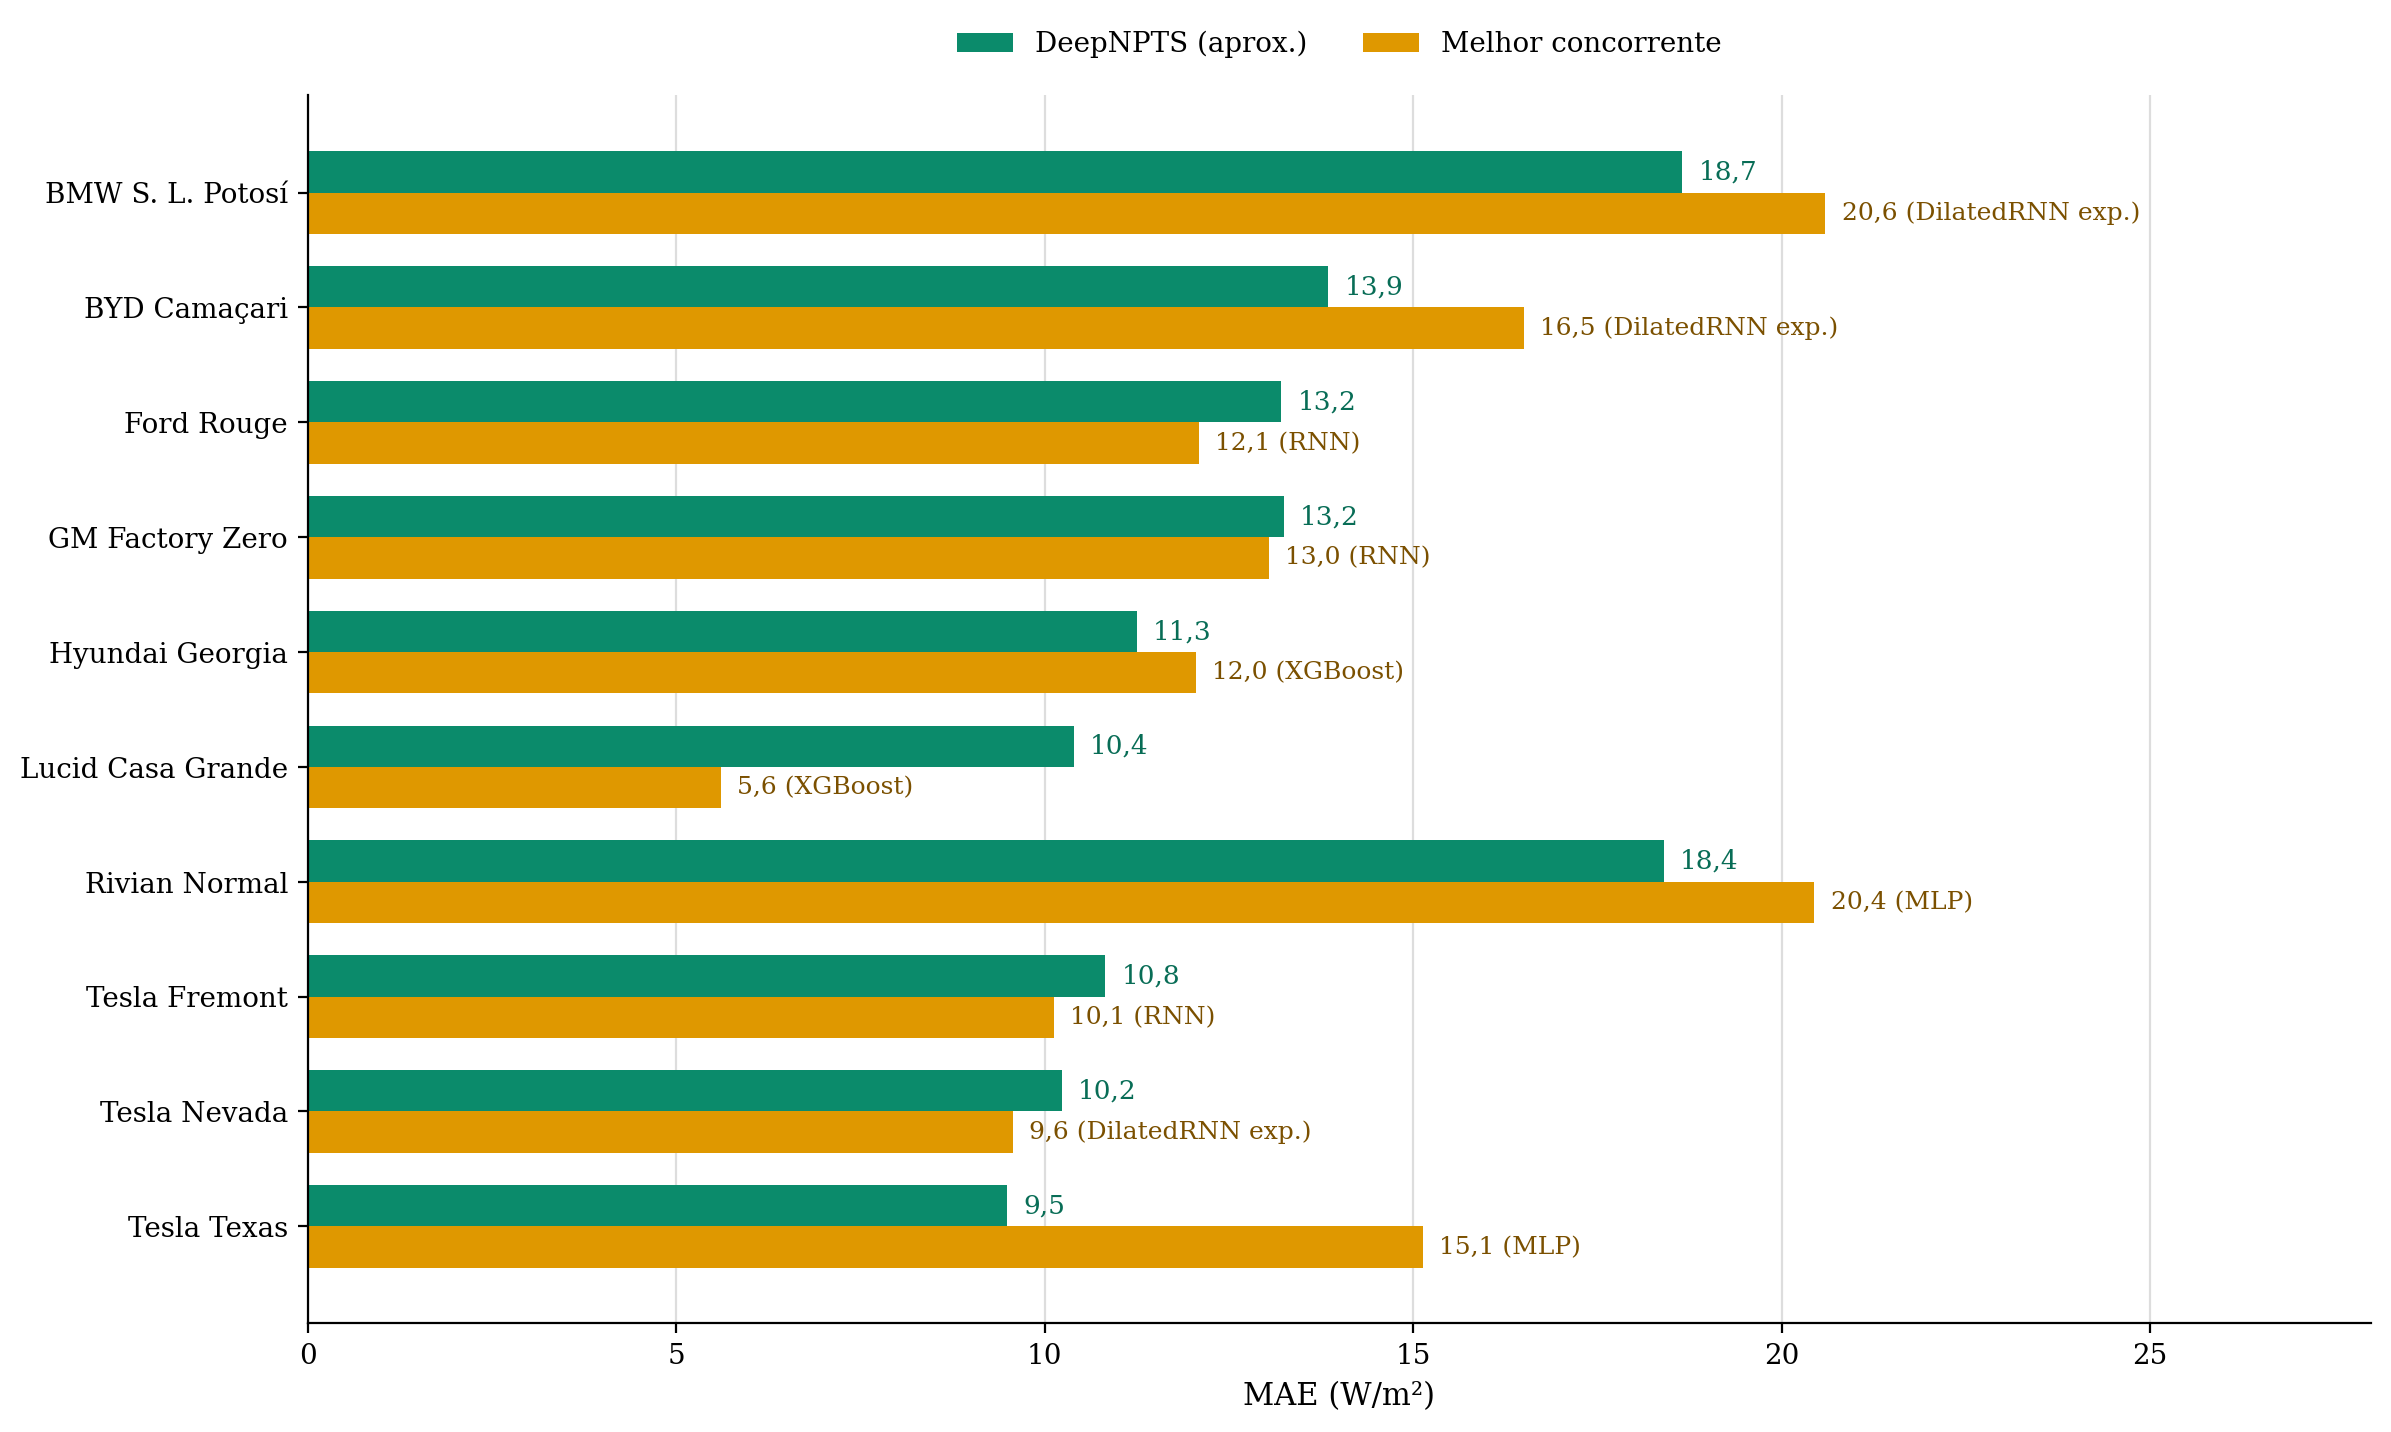
\includegraphics[width=0.96\textwidth]{mae_deepnpts_por_localidade_mcsm.png}
\caption{MAE da aproximação do DeepNPTS e do melhor concorrente em cada localidade.}
\label{fig:mae_localidades}
\end{figure}

\section{Conclusões}
\label{sec:conclusoes}

Este trabalho apresentou um sistema para previsão mensal de GHI baseado em uma aproximação experimental do DeepNPTS. O fluxo integrou aquisição, limpeza, agregação mensal, quantização, normalização, atributos temporais, divisão cronológica e comparação homogênea de sete modelos em dez localidades.

A aproximação foi a campeã geral, com MAE de 12,96 W/m$^2$, RMSE de 16,39 W/m$^2$, $R^2$ de 0,916 e nRMSE de 8,10\%. Frente à RNN, melhor referência média, as reduções foram de 12,50\% no MAE e 10,07\% no RMSE. O método venceu em cinco localidades, mas sua superioridade não foi uniforme, indicando que características regionais ainda influenciam a escolha do modelo.

Os resultados sustentam a ponderação por similaridade e recência como alternativa competitiva para séries mensais curtas. Trabalhos futuros devem empregar validação temporal em múltiplas janelas, repetir os modelos estocásticos, incluir variáveis meteorológicas, avaliar horizontes superiores a um mês e implementar o DeepNPTS canônico com treinamento conjunto de séries relacionadas.

\vspace{12pt}
\noindent\textbf{\textit{Agradecimentos.}} Os autores agradecem à FAPEMIG (processo OET-00243-26), à Universidade Estadual de Campinas (UNICAMP) e à Faculdade de Engenharia Elétrica e de Computação (FEEC) pelo apoio ao desenvolvimento deste projeto.

\begin{thebibliography}{99}

\bibitem[Antonanzas et al.(2016)]{antonanzas2016}
Antonanzas, J. et al. (2016), ``Review of photovoltaic power forecasting'', \textit{Solar Energy}, vol. 136, p. 78--111.

\bibitem[Chang et al.(2017)]{chang2017}
Chang, S. et al. (2017), ``Dilated recurrent neural networks'', \textit{Advances in Neural Information Processing Systems}.

\bibitem[Chen e Guestrin(2016)]{chen2016}
Chen, T. e Guestrin, C. (2016), ``XGBoost: A scalable tree boosting system'', \textit{Proceedings of the 22nd ACM SIGKDD International Conference on Knowledge Discovery and Data Mining}, p. 785--794.

\bibitem[Duffie e Beckman(2013)]{duffie2013}
Duffie, J.A. e Beckman, W.A. (2013), \textit{Solar Engineering of Thermal Processes}, 4a ed., Wiley, Hoboken.

\bibitem[Hochreiter e Schmidhuber(1997)]{hochreiter1997}
Hochreiter, S. e Schmidhuber, J. (1997), ``Long short-term memory'', \textit{Neural Computation}, vol. 9, n. 8, p. 1735--1780.

\bibitem[Hyndman e Koehler(2006)]{hyndman2006}
Hyndman, R.J. e Koehler, A.B. (2006), ``Another look at measures of forecast accuracy'', \textit{International Journal of Forecasting}, vol. 22, n. 4, p. 679--688.

\bibitem[National Laboratory of the Rockies(2026)]{nlr2026}
National Laboratory of the Rockies (2026), ``GOES Aggregated: PSM v4 Download API''. Disponível em: \url{https://developer.nlr.gov/docs/solar/nsrdb/nsrdb-GOES-aggregated-v4-0-0-download/}. Acesso em: 14 jul. 2026.

\bibitem[Rangapuram et al.(2023)]{rangapuram2023}
Rangapuram, S.S. et al. (2023), ``Deep non-parametric time series forecaster'', \textit{arXiv preprint arXiv:2312.14657}.

\bibitem[Salinas et al.(2020)]{salinas2020}
Salinas, D.; Flunkert, V.; Gasthaus, J. e Januschowski, T. (2020), ``DeepAR: Probabilistic forecasting with autoregressive recurrent networks'', \textit{International Journal of Forecasting}, vol. 36, n. 3, p. 1181--1191.

\bibitem[Sengupta et al.(2018)]{sengupta2018}
Sengupta, M. et al. (2018), ``The National Solar Radiation Data Base (NSRDB)'', \textit{Renewable and Sustainable Energy Reviews}, vol. 89, p. 51--60.

\bibitem[Sobri et al.(2018)]{sobri2018}
Sobri, S.; Koohi-Kamali, S. e Rahim, N.A. (2018), ``Solar photovoltaic generation forecasting methods: A review'', \textit{Energy Conversion and Management}, vol. 156, p. 459--497.

\bibitem[Voyant et al.(2017)]{voyant2017}
Voyant, C. et al. (2017), ``Machine learning methods for solar radiation forecasting: A review'', \textit{Renewable Energy}, vol. 105, p. 569--582.

\bibitem[Yang et al.(2018)]{yang2018}
Yang, D. et al. (2018), ``History and trends in solar irradiance and PV power forecasting'', \textit{Solar Energy}, vol. 168, p. 60--101.

\end{thebibliography}

\end{document}
